\section{Interfaces}

\begin{figure}
  \centering
  \begin{subfigure}[b]{0.22\textwidth}
    \fbox{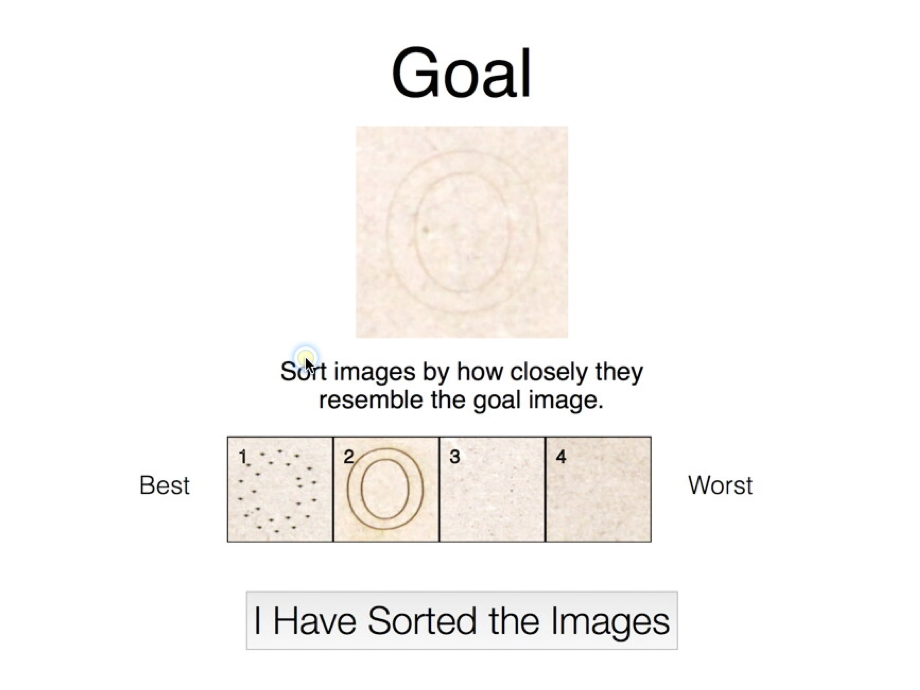
\includegraphics[width=\textwidth]{figures/interface_nm}}
    \caption{Nelder-Mead}\label{fig:interface_nm}
  \end{subfigure}
  \quad
  \begin{subfigure}[b]{0.22\textwidth}
    \fbox{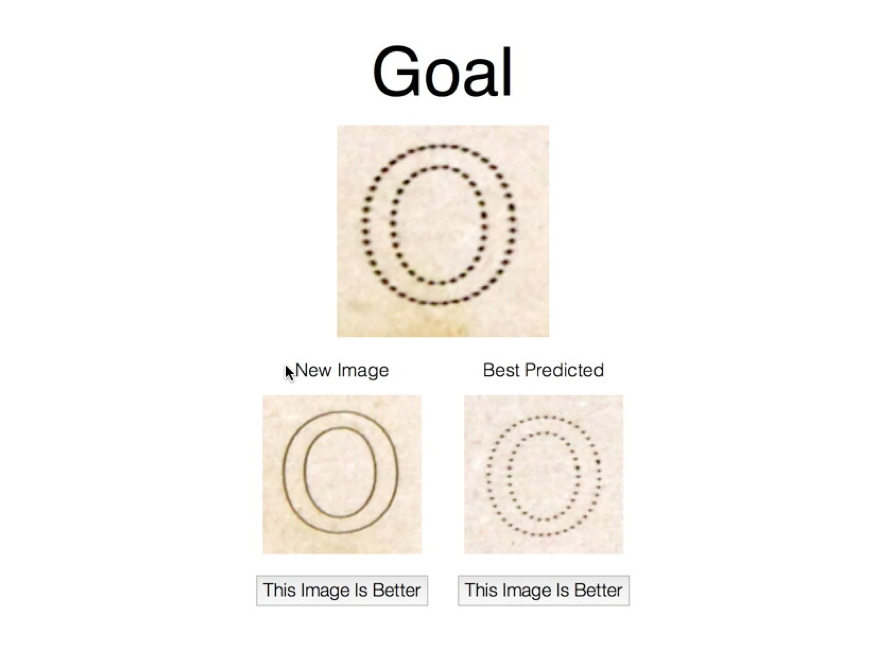
\includegraphics[width=\textwidth]{figures/interface_bo}}
    \caption{Bayesian Optimization}\label{fig:interface_bo}
  \end{subfigure}
  \caption{Interaces.}\label{fig:interfaces}
\end{figure}

\subsection{Nelder-Mead}

At each step, the Nelder-Mead algorithm needs to know which vertex in the simplex is the worst.
In some circumstances, it needs to know which one is the best, and which is second-to-worst.

All of these can be collected at once if a human provides a ranked list from best to worst of the quality of each of the points.
I built an interface to provide rankings to the Nelder-Mead algorithm (see Figure~\ref{fig:interface_nm}).
The output for each of the vertices is shown.
A human ranks each vertex by ordering their output---the images---from best to worst.
This is implemented with an ``insertion sort'' mechanism:
a user moves a vertex to a position in the list, and it displaces all vertexes to the right of it by moving them rightward.

When a user has finished ranking the examples, they click a button reporting they are finished.
The simplex then determines candidate next points (a reflection, expansion, or contraction) and presents these points within the list.
Based on the rank of the generated points, it determines whether to keep the new point or generate a different candidate point.

\subsection{Bayesian Optimization}

Brochu et al.'s variant on Bayesian optimization~\cite{brochu_tutorial_2010} suggests that an optimal point for an unknown cost function can be found by collecting comparison ratings between pairs of points.
In their implementation, a user was shown the best example seen so far, and an examples with the highest expected improvement.
Each ranking would be used to update both the best example seen so far, and the model for choosing a point based on expected improvement.

My interface for Bayesian Optimization is similar to Brochu et al.'s (see Figure~\ref{fig:interface_bo}).
A user is shown the best rated example, and an example that maximizes the expected improvement.
With each rating, both the best rated example and that which maximizes expected imporvement are updated.
The goal is shown between the two examples for a point of reference towards which users work.
